\section{Transformation Rules (one at a time)}

\begin{myCenteredBox}[
    title={Vertical Shift Up/Down},
    colbacktitle=black!10!white,
    colback=white,
    coltitle=black, fonttitle={\Large\scshape},
    width=7in,
    ]
    \renewcommand{\arraystretch}{1.5}
    \begin{minipage}{0.34\linewidth}
        \centering{\Large   $g(x) = \myRoot{x} + \boldsymbol{k}$   }
    \end{minipage}
    \hfill\vline\hfill
    \begin{minipage}{0.65\linewidth}
        \setlength{\tabcolsep}{1em}
        \begin{tabular}{ ll }
            {\large $g(x) = \myRoot{x} + 3$ } & {\large $g(x) = \myRoot{x} - 2$ }\\
            $k=$\gap{3} & $k=$\gap{-2} \\ 
            shift \gap{up} by \gap{3} & shift \gap{down} by \gap{2} \\ 
            {
                \begin{tikzpicture}[
                    scale=0.25,
                    xaxe style/.style = { very thick, arrows={-{Straight Barb}}, label={}, },                 
                    yaxe style/.style = { very thick, arrows={-{Straight Barb}}, label={}, },                 
                ]
                \scriptsize
                \tkzInit[ xmax=6, xmin=-6,  ymax=6, ymin=-6, ]
                \tkzGrid
                \tkzDrawXY[label={},color=black,]
                % \tkzLabelX[orig=false,]
                % \tkzLabelY[orig=false,]
                \tkzFct[domain = 0:6,thick, solid]{sqrt(x)}
                \tkzText[right](5.8,2.5){\large $f$}
                %
                % \tkzFct[domain = -6:6, thick, dashed]{sqrt(x)+3}
                % \tkzText[right](2.5,4){\large$g$}
            \end{tikzpicture}
            } 
            &
            {
                \begin{tikzpicture}[
                    scale=0.25,
                    xaxe style/.style = { very thick, arrows={-{Straight Barb}}, label={}, },                 
                    yaxe style/.style = { very thick, arrows={-{Straight Barb}}, label={}, },                 
                ]
                \scriptsize
                \tkzInit[ xmax=6, xmin=-6,  ymax=6, ymin=-6, ]
                \tkzGrid
                \tkzDrawXY[label={},color=black,]
                % \tkzLabelX[orig=false,]
                % \tkzLabelY[orig=false,]
                \tkzFct[domain = 0:6,thick, solid]{sqrt(x)}
                \tkzText[right](5.8,2.5){\large $f$}
                %
                % \tkzFct[domain = -6:6, thick, dashed]{sqrt(x)-2}
                % \tkzText[right](6,1){\large$g$}
            \end{tikzpicture}
            } 
            \\
        \end{tabular}
    \end{minipage}
\end{myCenteredBox}
\begin{myCenteredBox}[
    title={Horizontal Shift Left/Right},
    colbacktitle=black!10!white,
    colback=white,
    coltitle=black, fonttitle={\Large\scshape},
    width=7in,
    ]
    \renewcommand{\arraystretch}{1.5}
    \begin{minipage}{0.29\linewidth}
        \centering{\Large   $g(x) = \myRoot{x-\boldsymbol{h}} $   }
    \end{minipage}
    \hfill\vline\hfill
    \begin{minipage}{0.7\linewidth}
        \setlength{\tabcolsep}{1em}
        \begin{tabular}{ ll }
            {\large $g(x) = \myRoot{x-5} $ } & {\large $g(x) = \myRoot{x+4} $ } \\ 
            $h=$\gap{5} & $h=-$\gap{4} \\ 
            shift \gap{right} by \gap{5}  & shift \gap{left} by \gap{4} \\ 
            {
                \begin{tikzpicture}[
                    scale=0.25,
                    xaxe style/.style = { very thick, arrows={-{Straight Barb}}, label={}, },                 
                    yaxe style/.style = { very thick, arrows={-{Straight Barb}}, label={}, },                 
                ]
                \scriptsize
                \tkzInit[ xmax=10, xmin=-2,  ymax=6, ymin=-6, ]
                \tkzGrid
                \tkzDrawXY[label={},color=black,]
                % \tkzLabelX[orig=false,]
                % \tkzLabelY[orig=false,]
                \tkzFct[domain = 0:10,thick, solid]{sqrt(x)}
                \tkzText[right](10,2.5){\large $f$}
                %
                % \tkzFct[domain = -6:10, thick, dashed]{sqrt(x-5)}
                % \tkzText[right](4,-1){\large$g$}
            \end{tikzpicture}
            } 
            &
            {
                \begin{tikzpicture}[
                    scale=0.25,
                    xaxe style/.style = { very thick, arrows={-{Straight Barb}}, label={}, },                 
                    yaxe style/.style = { very thick, arrows={-{Straight Barb}}, label={}, },                 
                ]
                \scriptsize
                \tkzInit[ xmax=6, xmin=-6,  ymax=6, ymin=-6, ]
                \tkzGrid
                \tkzDrawXY[label={},color=black,]
                % \tkzLabelX[orig=false,]
                % \tkzLabelY[orig=false,]
                \tkzFct[domain = 0:6,thick, solid]{sqrt(x)}
                \tkzText[right](5.8,2.5){\large $f$}
                %
                % \tkzFct[domain = -6:6, thick, dashed]{sqrt(x+4)}
                % \tkzText[right](2.5,4){\large$g$}
            \end{tikzpicture}
            } \\
        \end{tabular}
    \end{minipage}

    \vspace{0.5em}
    $h$ is the \gap{opposite} of what you see.
\end{myCenteredBox}
\begin{myCenteredBox}[
    title={Vertical Stretch/Compression},
    colbacktitle=black!10!white,
    colback=white,
    coltitle=black, fonttitle={\Large\scshape},
    width=7in,
]
    \renewcommand{\arraystretch}{1.5}
    \begin{minipage}{0.28\linewidth}
    \centering{   \Large $g(x) = \boldsymbol{a} \myRoot{x} $   }
    \end{minipage}
    \hfill\vline\hfill
    \begin{minipage}{0.71\linewidth}
    \setlength{\tabcolsep}{1em}
    \begin{tabular}{ ll }
        {\large $g(x) = 2 \myRoot{x} $ } & {\large $g(x) = \frac{1}{2} \myRoot{x} $} \\
        %
        $a=$\gap{2} & $a=$\gap{1/2} \\ 
        %
        stretch by a factor of \gap{5} & compress by a factor of \gap{$1/2$} \\ 
        {
            \begin{tikzpicture}[
                scale=0.25,
                xaxe style/.style = { very thick, arrows={-{Straight Barb}}, label={}, },                 
                yaxe style/.style = { very thick, arrows={-{Straight Barb}}, label={}, },                 
                ]
                \scriptsize
                \tkzInit[ xmax=6, xmin=-6,  ymax=6, ymin=-6, ]
                \tkzGrid
                \tkzDrawXY[label={},color=black,]
                % \tkzLabelX[orig=false,]
                % \tkzLabelY[orig=false,]
                \tkzFct[domain = 0:6,thick, solid]{sqrt(x)}
                \tkzText[right](5.8,2.5){\large $f$}
                %
                % \tkzFct[domain = -6:6, thick, dashed]{2*sqrt(x)}
                % \tkzText[right](5.8,5){\large$g$}
            \end{tikzpicture}
            } 
            &
            {
                \begin{tikzpicture}[
                    scale=0.25,
                    xaxe style/.style = { very thick, arrows={-{Straight Barb}}, label={}, },                 
                    yaxe style/.style = { very thick, arrows={-{Straight Barb}}, label={}, },                 
                ]
                \scriptsize
                \tkzInit[ xmax=6, xmin=-6,  ymax=6, ymin=-6, ]
                \tkzGrid
                \tkzDrawXY[label={},color=black,]
                % \tkzLabelX[orig=false,]
                % \tkzLabelY[orig=false,]
                \tkzFct[domain = 0:6,thick, solid]{sqrt(x)}
                \tkzText[right](5.8,2.5){\large $f$}
                %
                % \tkzFct[domain = -6:6, thick, dashed]{0.5*sqrt(x)}
                % \tkzText[right](5.8,1){\large$g$}
            \end{tikzpicture}
            } 
            \\
        \end{tabular}
    \end{minipage}

    \vspace{0.5em}
    {\bfseries\itshape Vertical stretch} when \gap{$a>1$}

    \vspace{0.5em}
    {\bfseries\itshape Vertical compress} when \gap{$0<a<1$}
\end{myCenteredBox}
\begin{myCenteredBox}[
    title={Reflection},
    colbacktitle=black!10!white,
    colback=white,
    coltitle=black, fonttitle={\Large\scshape},
    width=7in,
    ]
    \renewcommand{\arraystretch}{1.5}
    \begin{minipage}{0.49\linewidth}
        \centering{   \Large $g(x) = \boldsymbol{a} \myRoot{x} $   }
    \end{minipage}
    \begin{minipage}{0.49\linewidth}
        \begin{tabular}{c}
            {\large $g(x) = - \myRoot{x} $ } 
            \\
            $a=$\gap{-1} 
            \\
            reflection across the \gap{$x$-axis}
            \\
            \begin{tikzpicture}[
                scale=0.25,
                xaxe style/.style = { very thick, arrows={-{Straight Barb}}, label={}, },                 
                yaxe style/.style = { very thick, arrows={-{Straight Barb}}, label={}, },                 
                ]
                \scriptsize
                \tkzInit[ xmax=6, xmin=-6,  ymax=6, ymin=-6, ]
                \tkzGrid
                \tkzDrawXY[label={},color=black,]
                % \tkzLabelX[orig=false,]
                % \tkzLabelY[orig=false,]
                \tkzFct[domain = 0:6,thick, solid]{sqrt(x)}
                \tkzText[right](5.8,2.5){\large $f$}
                %
                % \tkzFct[domain = -6:6, thick, dashed]{-sqrt(x)}
                % \tkzText[right](5.8,-2.5){\large$g$}
            \end{tikzpicture}
            \\
        \end{tabular}
    \end{minipage}

    \vspace{1\baselineskip}
    When $a$ is \gap{negative}, there is a \gap{reflection} across the $x$-axis.
\end{myCenteredBox}